\documentclass[]{homework}

\usepackage{tikz}
\usetikzlibrary{decorations.pathreplacing}

% \usepackage[]{floatflt}
\usepackage{wrapfig}

\begin{document}

\homework{1}{Jan. 28, 2021}


\begin{problem}{0}

  {\em If you're already familiar with Python and Jupyter notebooks, you may skip this problem. Otherwise,
  you should complete this problem ASAP!}

  This ``problem'' is a couple of tasks you must complete during the first week of classes.
  The sooner you do, the better!

  Becoming comfortable with the tools we will be using is important and can only be acquired through practice.
  
  \begin{subproblem}{a}
    Install Python and jupyter. 
    You may use this for the homeworks, labs, and exams, and it will also be useful for running example notebooks.
    More details can be found through the \emph{Python Information} page on Canvas.
    Unless you are certain you know better, install the Python 3 version of the Anaconda distribution.
  \end{subproblem}

  \begin{subproblem}{b}
    Watch the \href{https://www.youtube.com/watch?v=DKiI6NfSIe8}{introductory video} on the Jupyter notebook.
    Information about the video can also be found on the \emph{Python Information} page on Canvas.
  \end{subproblem}

\end{problem}


% \begin{wrapfigure}{r}{3cm}

% \end{wrapfigure}


\begin{problem}{1}
  A square is constructed with sides of unit length. Subsequent square are nested 
  inside by constructing them
  from vertexes placed at the midpoints of their parent squares, as shown in the figure below right.

  \begin{subproblem}{a}
    \begin{minipage}[t]{\linewidth}
      \begin{wrapfigure}{r}{3cm}
        \vspace{-1em}
        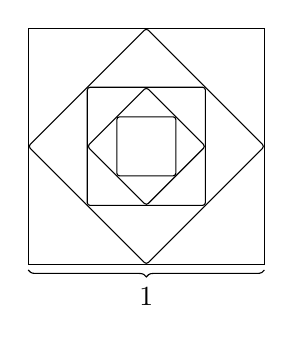
\begin{tikzpicture}
          \def\rectlen{3cm}
          \def\rectnum{4}
          \path[coordinate] (0,0) coordinate (A)
            ++(\rectlen,0) coordinate (B)
            ++(0,\rectlen) coordinate (C)
            ++(-\rectlen,0) coordinate (D);
          \draw[] (A) -- (B) -- (C) -- (D) -- cycle;
          \draw[decorate,decoration={brace,raise=2pt}] (B) -- (A)
            node [midway,below,yshift=-5pt] {$1$};
          \foreach \junk in {1,...,\rectnum}{%
            \path[coordinate] coordinate(X) at (A){};
            \path[coordinate] (A) -- (B) coordinate[pos=0.5] (A)
              -- (C) coordinate[pos=0.5] (B)
              -- (D) coordinate[pos=0.5] (C)
              -- (X) coordinate[pos=0.5] (D);
            \draw[rounded corners=1pt] (A) -- (B) -- (C) -- (D) -- cycle;
          }
        \end{tikzpicture}
      \end{wrapfigure}
      \vspace{-0.7  em}
      Write the sum of the perimeters of the squares.
      This is a geometric series, so we can calculate the sum analytically!
      For $N$ squares what is the sum?
      For $N\rightarrow\infty$ what is the sum?
      \note{For one square ($N=1$) you know the perimeter.
      Does your expression agree?
      If not, you may have an ``off by one'' error.}
    \end{minipage}
  \end{subproblem}
  \begin{subproblem}{b}
    Repeat the previous part for the sum of the areas of the squares.
  \end{subproblem}
  \begin{subproblem}{c}
    Numerically we cannot perform the sum to infinity so it must be truncated; this leads to an error in our calculation.
    Derive formulas for the number of terms required to evaluate the sums from the previous two parts to an accuracy $\epsilon$.\\
    \hint{If we know the true perimeter $p$, and the sum truncated after summing over $N$ terms, $p_N$, what is $N$ such that $|p - p_N| < \epsilon$?}
  \end{subproblem}
  \begin{subproblem}{d}
    For an accuracy of $\epsilon=10^{-7}$, how many terms will be required?
    Verify this by performing the sums numerically.
    Do the results agree?
    It is also interesting to consider the case when $\epsilon=10^{-15}$.  In particular, what happens for the perimeter calculation? Can you explain why this happens?
  \end{subproblem}
\end{problem}


\begin{problem}{2}
  Complete the Jupyter notebook assignment.
\end{problem}


\end{document}

